\item In the arrangement shown in Fig. 1.17 the mass of the rod \( M \) exceeds the mass \( m \) of the ball. The ball has an opening permitting it to slide along the thread with some friction. 
    \begin{center}
        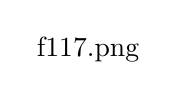
\begin{tikzpicture}
            \node at (0, 0) {{f117.png}};
        \end{tikzpicture}
    \end{center}
    The mass of the pulley and the friction in its axle are negligible. At the initial moment the ball was located opposite the lower end of the rod. When set free, both bodies began moving with constant accelerations. Find the friction force between the ball and the thread at \( t \) seconds after the beginning of motion the ball got opposite the upper end of the rod. The rod length equals \( l \).
\begin{solution}
    \begin{center}
        \begin{tikzpicture}
            \pic at (0, 0) {frame=3cm};
        \end{tikzpicture}
    \end{center}
    
    \begin{align*}
        \intertext{As the thread is not tied with \( m \), so if there were no friction between the thread and the ball \( m \), the tension in the thread would be zero and as a result both bodies will have free fall motion. Obviously in the given problem it is the friction force exerted by the ball on the thread, which becomes the tension in the thread. From the condition or language of the problem \( w_M > w_m \) and as both are directed downward so, relative acceleration of \( M = w_M - w_m \) and is directed downward.}
        \intertext{Kinematical equation for the ball in the frame of rod in projection form along upward direction gives}
        l &= \dfrac{1}{2} \left( w_M - w_m \right) t^2 \tag{1}\\
        \intertext{Newton’s second law in projection form along vertically down direction for both, rod and ball gives,}
        Mg - f_r &= Mw_M \tag{2}\\
        mg - f_r &= mw_m \tag{3}\\
        \intertext{Multiplying Eq. (2) by \( m \) and Eq. (3) by \( M \) and then subtracting Eq. (3) from Eq. (2) and after using Eq. (1), we get}
        f_r &= \dfrac{2l\,M\,m}{(M - m) t^2}
    \end{align*}
\end{solution}
